\documentclass[12pt,a4paper]{article}
\usepackage{amsmath,amsfonts,amssymb}
\usepackage{graphicx}
\usepackage{enumitem}
\usepackage[dvipsnames]{xcolor}
\usepackage{pgfplots}
\usepackage{hyperref}
\usepackage{soul}
\usepackage{framed}
\usepackage{booktabs} 
\usepackage{tabularx}
\usepackage{array}


\definecolor{lessonbgcolor}{rgb}{0.9,0.9,1}
\definecolor{examplecolor}{rgb}{0.8,1,0.8}
\definecolor{noteboxcolor}{rgb}{1,0.8,0.8}
\newenvironment{lesson}[1]
  {\begin{framed}\colorbox{lessonbgcolor}{
  \parbox{\dimexpr\linewidth-2\fboxsep}{
  \textbf{#1}}}\end{framed}}
  
\newenvironment{example}
  {\begin{framed}\colorbox{examplecolor}{
  \parbox{\dimexpr\linewidth-2\fboxsep}{
  \textbf{Example:}}}}
  {\end{framed}}
\newenvironment{note}
  {\begin{framed}\colorbox{noteboxcolor}{
  \parbox{\dimexpr\linewidth-2\fboxsep}{
  \textbf{Note:}}}}
  {\end{framed}}

\pgfplotsset{width=7cm,compat=1.17}
\title{Grade 11 Functions Notes: Unit 1}
\author{Made By Kensukeken}
\date{\today}

\begin{document}
\maketitle

\section*{Unit 1: Intro To Functions}

\subsection*{Lesson 1 - Domain and Range}
The domain and range of a function describe the possible input and output values, respectively.



\textbf{\hl{Example 1:}} For \(f(x) = \sqrt{x}\), the domain is \(x \geq 0\) since you can't take the square root of a negative number without delving into complex numbers.

\textbf{\hl{Example 2:}} For \(f(x) = \frac{1}{x}\), the domain is \(x \neq 0\) since division by zero is undefined.

\textbf{\hl{Example 3:}} For a parabola \(f(x) = x^2\), the range is \(f(x) \geq 0\).

\subsection*{Lesson 2 - Function Notation}
Function notation introduces a more concise way to represent equations.

\textbf{\hl{Example 1:}} Given \(f(x) = 2x^2 + 3\), find \(f(2)\). Solution: \(f(2) = 2(2^2) + 3 = 11\).

\textbf{\hl{Example 2:}} If \(f(x) = x + 5\), what is \(f(3)\)? Solution: \(f(3) = 3 + 5 = 8\).

\textbf{Function Table for \(f(x) = x^2\)}:
\begin{center}
    \begin{tabular}{c|c}
        \( x \) & \( f(x) \) \\
        \hline
        -2 & 4 \\
        -1 & 1 \\
        0 & 0 \\
        1 & 1 \\
        2 & 4 \\
    \end{tabular}
\end{center}
\newpage
\subsection*{Lesson 3 - Max/Min of Quadratics}
The vertex of a quadratic function indicates its maximum or minimum value.
\subsubsection*{Properties of Quadratic Expressions}

Quadratic expressions, depending on their leading coefficients, have certain inherent properties:

\begin{enumerate}
    \item Any square of a number, \(x^2\), is always non-negative. Thus, \(x^2 \geq 0\). This is because squaring any real number, whether positive or negative, results in a positive value (or zero if \(x = 0\)).
    
    \item The negative of a square, \(-x^2\), is always non-positive. Thus, \(-x^2 \leq 0\). This is the opposite behavior of \(x^2\), as negating it ensures the parabola opens downward.
    
    \item For a quadratic in the form of \(-(x-h)^2\), where \(h\) is a constant, the expression represents a downward-opening parabola shifted \(h\) units to the right on the x-axis. As an example, for \(-(x-4)^2\), the parabola is shifted 4 units to the right, and \(-(x-4)^2 \leq 0\).
\end{enumerate}

\textbf{Note:} The sign and nature of the leading coefficient in a quadratic expression can give insights into the orientation of the parabola and its range.

\textbf{\hl{Example 1:}} Find the vertex of \(f(x) = 2x^2 + 4x + 3\). By completing the square, the vertex is \((-1, 1)\).

\textbf{\hl{Example 2:}} For \(f(x) = -x^2 + 4x - 3\), the vertex is \((2, 5)\) and represents a maximum due to the negative leading coefficient.

\subsection*{Lesson 4 - Radicals}
Radicals involve taking roots of numbers.

\textbf{\hl{Example 1:}} Simplify \(\sqrt[3]{27}\). Solution: \(3\).

\textbf{\hl{Example 2:}} Simplify \(\sqrt{81}\). Solution: \(9\).

\textbf{\hl{Example 3:}} Determine the domain of \(f(x) = \sqrt{x - 5}\). Solution: \(x \geq 5\).

\subsection*{Lesson 5 - Solve Quadratics by Factoring}
Factoring is a method to solve quadratic equations.

\textbf{\hl{Example 1:}} Solve \(x^2 - 5x + 6 = 0\). Solution: \((x - 2)(x - 3) = 0\), so \(x = 2\) or \(x = 3\).

\textbf{\hl{Example 2:}} Solve \(x^2 - x - 6 = 0\). Solution: \((x - 3)(x + 2) = 0\), so \(x = 3\) or \(x = -2\).

\subsection*{Lesson 6 - Quadratic Formula}
When factoring is not possible, the quadratic formula offers a solution.

\textbf{Formula:}
\[x = \frac{-b \pm \sqrt{b^2 - 4ac}}{2a}\]

\textbf{\hl{Example:}} Solve \(x^2 + x - 1 = 0\). Plugging the coefficients into the formula will give two solutions for \(x\).

\subsection*{Lesson 7 - Linear Quadratic Systems}

Linear Quadratic Systems involve a combination of linear and quadratic equations. Solving these systems can reveal points of intersection between the two functions, if they exist.

\textbf{Methods of Solution:}
\begin{enumerate}
    \item \textbf{Substitution:} Use the linear equation to solve for \(y\) (or \(x\)), and then substitute this expression into the quadratic equation.
    \item \textbf{Graphical:} Graph both the linear and quadratic functions on the same set of axes and identify the point(s) of intersection.
\end{enumerate}

\textbf{\hl{Example 1:}} Solve the system:
\[
\begin{aligned}
    y &= x^2 + 2 \\
    y &= 2x + 3
\end{aligned}
\]

By substitution, set \(x^2 + 2\) equal to \(2x + 3\). Solving this equation will give the \(x\)-coordinates of the intersection points. To find the corresponding \(y\)-coordinates, substitute these \(x\)-values into either the linear or quadratic equation.

\textbf{\hl{Example 2:}} Solve the system:
\[
\begin{aligned}
    y &= x^2 - 4 \\
    y &= -x + 2
\end{aligned}
\]

Again, using substitution, equate \(x^2 - 4\) to \(-x + 2\). This will yield the \(x\)-coordinates of where the line intersects the parabola. To find the corresponding \(y\)-values, plug these \(x\)-values into one of the original equations.

\textbf{Note:} Sometimes, a linear function might not intersect a quadratic function, or it might intersect at one or two points. The nature of intersection can also be discerned graphically or by assessing the discriminant when setting the two equations equal to each other.

\subsection*{Translations and Function Notation}

Given a function \( y = f(x) \), the following transformations can be applied:

\begin{itemize}
    \item \textbf{Vertical Translation:} \( y = f(x) + c \) shifts the graph \(c\) units upward (if \(c > 0\)) or downward (if \(c < 0\)).
    \item \textbf{Horizontal Translation:} \( y = f(x - h) \) shifts the graph \(h\) units to the right (if \(h > 0\)) or to the left (if \(h < 0\)).
    \item \textbf{Vertical Stretch/Compression:} \( y = af(x) \) stretches the graph by a factor of \(a\) if \(a > 1\), or compresses it if \(0 < a < 1\). If \(a < 0\), the graph is also reflected about the x-axis.
    \item \textbf{Horizontal Stretch/Compression:} \( y = f(bx) \) compresses the graph horizontally by a factor of \(b\) if \(b > 1\), or stretches it if \(0 < b < 1\).
\end{itemize}

A translation is a type of transformation that changes the location of a function in the coordinate plane, while preserving its shape and size.

\subsubsection*{Representation Using Function Notation}
Translations can be represented using function notation:
\[ y = f(x - h) + k \]
This represents the function \( y = f(x) \) translated horizontally by \( h \) units and vertically by \( k \) units.

\begin{itemize}
    \item If \( h > 0 \), the function is translated to the right.
    \item If \( h < 0 \), the function is translated to the left.
    \item If \( k > 0 \), the function is translated up.
    \item If \( k < 0 \), the function is translated down.
\end{itemize}

\subsubsection*{Sketching Translated Graphs}
To sketch the graph of \( y = f(x - h) + k \), start with the graph of \( f(x) \) and translate points on that function based on the values of \( h \) and \( k \). Asymptotes, if any, must also be translated.

\subsubsection*{Translations of Common Base Functions}
\vspace*{\fill}
\[
\begin{tabular}{|c|c|}
    \hline
    \textcolor{Orchid}{Base Function} & \textcolor{WildStrawberry}{Translated Function} \\
    \hline
    \( f(x) = x^2 \) & \( y = (x - h)^2 + k \) \\
    \hline
    \( f(x) = \sqrt{x} \) & \( y = \sqrt{x - h} + k \) \\
    \hline    
    \( f(x) = \frac{1}{x} \) & \( y = \frac{1}{x - h} + k \) \\
    \hline
\end{tabular}
\]
\vspace*{\fill}

\subsubsection*{$\bigstar$ Domain and Range}
When a function is translated, the domain and range of the function are translated as well.


\subsection*{\textcolor{blue}{Examples}}

\textbf{\hl{Example 1:}} Consider the function \(y = \sqrt{x}\).

\textbf{Transformation:} The graph of \(y = 2\sqrt{x-3} + 1\):

\begin{itemize}
    \item Starts with the basic square root graph.
    \item Stretches vertically by a factor of 2.
    \item Translates 3 units to the right.
    \item Translates 1 unit upwards.
\end{itemize}

\textbf{Description:} This graph will resemble the basic upward curving square root graph, but will be steeper (due to the vertical stretch), and shifted to the point (3,1) as its starting point.

\textbf{\hl{Example 2:}} Consider the function \(y = x^2\).

\textbf{Transformation:} The graph of \(y = -0.5(x+2)^2 - 4\):

\begin{itemize}
    \item Starts with the basic parabolic graph.
    \item Reflects about the x-axis (due to the negative sign).
    \item Compresses vertically by a factor of 0.5.
    \item Translates 2 units to the left.
    \item Translates 4 units downward.
\end{itemize}

\textbf{Description:} This graph will resemble an upside-down parabola, opening downward, being wider than the standard \(y = x^2\) graph (due to the vertical compression), and having its vertex at the point (-2,-4).
\subsection*{\hl{Shortcut Words For Transformation}}
\begin{align*}
    & \text{\hl{VT}} \xrightarrow{} \text{Vertical Translation} \\
    & \text{\hl{HT}} \xrightarrow{} \text{Horizontal Translation} \\
    & \text{\hl{VS}} \xrightarrow{} \text{Vertical Stretch} \\
    & \text{\hl{HS}} \xrightarrow{} \text{Horizontal Stretch} \\
    & \text{\hl{RXA}} \xrightarrow{} \text{Reflection in x-axis} \\
    & \text{\hl{RYA}} \xrightarrow{} \text{Reflection in y-axis} \\
\end{align*}

\subsection*{Summary Lesson}

\[
\begin{array}{lll}
\text{Notation} & \text{Transformation Type} & \text{Coordinate Change} \\
\textcolor{CadetBlue}{f(x)+d} & \textcolor{CadetBlue}{\text{Vertical translation up } d \text{ units}} & (x, y) \mapsto(x, y+d) \\
\textcolor{CadetBlue}{f(x)-d} & \textcolor{CadetBlue}{\text{Vertical translation down } d \text{ units}} & (x, y) \mapsto(x, y-d) \\
\textcolor{CadetBlue}{f(x+c)} & \textcolor{CadetBlue}{\text{Horizontal translation left } c \text{ units}} & (x, y) \mapsto(x-c, y) \\
\textcolor{CadetBlue}{f(x-c)} & \textcolor{CadetBlue}{\text{Horizontal translation right } c \text{ units}} & (x, y) \mapsto(x+c, y) \\
\textcolor{CadetBlue}{-f(x)} & \textcolor{CadetBlue}{\text{Reflection over } x \text{-axis}} & (x, y) \mapsto(x,-y) \\
\textcolor{CadetBlue}{f(-x)} & \textcolor{CadetBlue}{\text{Reflection over } y \text{-axis}} & (x, y) \mapsto(-x, y) \\
\textcolor{CadetBlue}{a f(x)} & \textcolor{CadetBlue}{\text{Vertical stretch for } |a|>1} & (x, y) \mapsto(x, a y) \\
\textcolor{CadetBlue}{a f(x)} & \textcolor{CadetBlue}{\text{Vertical compression for } |a|<1} & (x, y) \mapsto(x, a y) \\
\textcolor{CadetBlue}{f(b x)} & \textcolor{CadetBlue}{\text{Horizontal compression for } |b|>1} & (x, y) \mapsto\left(\frac{x}{b}, y\right) \\
\textcolor{CadetBlue}{f(b x)} & \textcolor{CadetBlue}{\text{Horizontal stretch for } |b|<1} & (x, y) \mapsto\left(\frac{x}{b}, y\right)
\end{array}
\]


\newpage
\section*{\hl{Parent Functions}}

\subsection*{1. Linear Function: $f(x) = x$}
\begin{minipage}{0.5\textwidth}
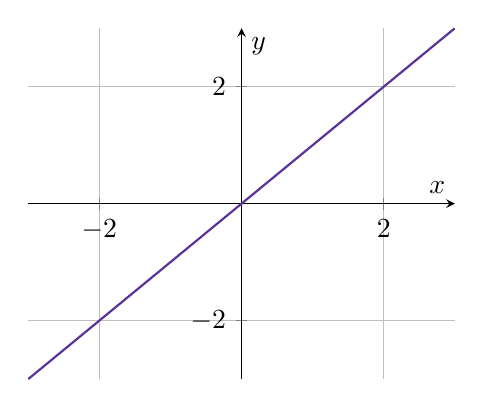
\begin{tikzpicture}
    \begin{axis}[
        grid=both,
        axis lines=middle,
        xmin=-3, xmax=3,
        ymin=-3, ymax=3,
        xlabel={$x$},
        ylabel={$y$},
        ]
        \addplot[RoyalPurple, thick, domain=-3:3] {x};
    \end{axis}
\end{tikzpicture}
\end{minipage}
\hspace{1cm}
\begin{minipage}{0.4\textwidth}
\centering
\begin{tabular}{cc}

$x$ & $f(x)$ \\
-2 & -2 \\
-1 & -1 \\
0 & 0 \\
1 & 1 \\
2 & 2 \\

\end{tabular}
\end{minipage}

The linear function $f(x) = x$ represents a \hl{straight line} that passes through the origin (0,0) and has a slope of 1. As $x$ increases or decreases, $f(x)$ increases or decreases respectively.

\subsection*{2. Quadratic Function: $f(x) = x^2$}
\begin{minipage}{0.5\textwidth}
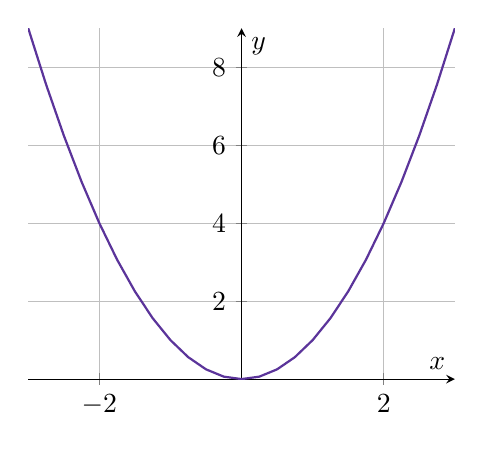
\begin{tikzpicture}
    \begin{axis}[
        grid=both,
        axis lines=middle,
        xmin=-3, xmax=3,
        ymin=0, ymax=9,
        xlabel={$x$},
        ylabel={$y$},
        ]
        \addplot[RoyalPurple, thick, domain=-3:3] {x^2};
    \end{axis}
\end{tikzpicture}
\end{minipage}
\hspace{1cm}
\begin{minipage}{0.4\textwidth}
\centering
\begin{tabular}{cc}
\toprule
$x$ & $f(x)$ \\

-2 & 4 \\
-1 & 1 \\
0 & 0 \\
1 & 1 \\
2 & 4 \\

\end{tabular}
\end{minipage}

The quadratic function $f(x) = x^2$ represents a parabola that opens upwards and has \hl{its vertex} at the origin (0,0). The function values are always non-negative and increase quadratically as $x$ moves away from 0.

\subsection*{3. Cubic Function: $f(x) = x^3$}
\begin{minipage}{0.5\textwidth}
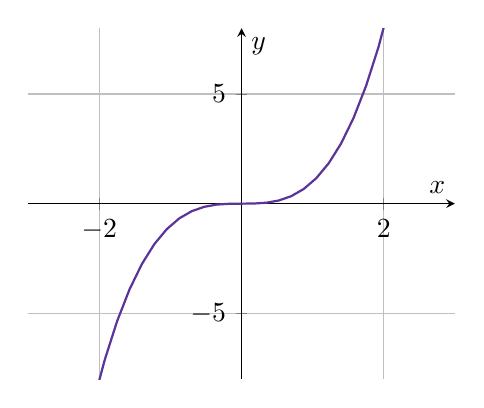
\begin{tikzpicture}
    \begin{axis}[
        grid=both,
        axis lines=middle,
        xmin=-3, xmax=3,
        ymin=-8, ymax=8,
        xlabel={$x$},
        ylabel={$y$},
        ]
        \addplot[RoyalPurple, thick, domain=-2.1:2.1] {x^3};
    \end{axis}
\end{tikzpicture}
\end{minipage}
\hspace{1cm}
\begin{minipage}{0.4\textwidth}
\centering
\begin{tabular}{cc}

$x$ & $f(x)$ \\

-2 & -8 \\
-1 & -1 \\
0 & 0 \\
1 & 1 \\
2 & 8 \\
\end{tabular}
\end{minipage}

The cubic function $f(x) = x^3$ has a characteristic \hl{S-shape} and crosses the origin (0,0). The function values increase cubically as $x$ moves away from 0, with $f(x)$ being negative when $x$ is negative and positive when $x$ is positive.

\subsection*{4. Reciprocal Function: $f(x) = \frac{1}{x}$}
\begin{minipage}{0.5\textwidth}
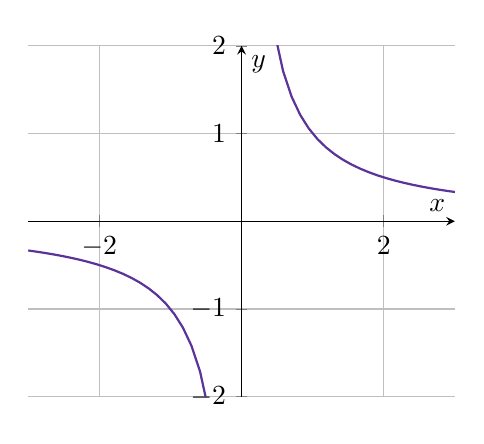
\begin{tikzpicture}
    \begin{axis}[
        grid=both,
        axis lines=middle,
        xmin=-3, xmax=3,
        ymin=-2, ymax=2,
        xlabel={$x$},
        ylabel={$y$},
        ]
        \addplot[RoyalPurple, thick, domain=-3:-0.1] {1/x};
        \addplot[RoyalPurple, thick, domain=0.1:3] {1/x};
    \end{axis}
\end{tikzpicture}
\end{minipage}
\hspace{1cm}
\begin{minipage}{0.4\textwidth}
\centering
\begin{tabular}{cc}

$x$ & $f(x)$ \\

-3 & -0.33 \\
-2 & -0.5 \\
-1 & -1 \\
1 & 1 \\
2 & 0.5 \\
3 & 0.33 \\

\end{tabular}
\end{minipage}
\noindent
The reciprocal function $f(x) = \frac{1}{x}$ has \hl{two hyperbolas} in the 1st and 3rd quadrants. As $x$ approaches 0 from either side, $f(x)$ approaches $\pm\infty$. 

\subsection*{5. Square Root Function: $f(x) = \sqrt{x}$}
\begin{minipage}{0.5\textwidth}
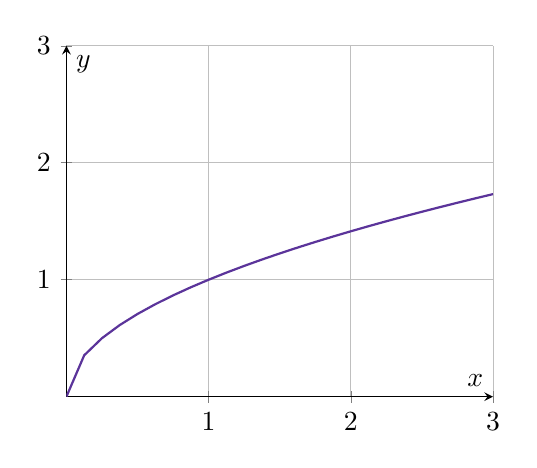
\begin{tikzpicture}
    \begin{axis}[
        grid=both,
        axis lines=middle,
        xmin=0, xmax=3,
        ymin=0, ymax=3,
        xlabel={$x$},
        ylabel={$y$},
        ]
        \addplot[RoyalPurple, thick, domain=0:3] {sqrt(x)};
    \end{axis}
\end{tikzpicture}
\end{minipage}
\hspace{1cm}
\begin{minipage}{0.4\textwidth}
\centering
\begin{tabular}{cc}
\toprule
$x$ & $f(x)$ \\

0 & 0 \\
1 & 1 \\
2 & 1.41 \\
3 & 1.73 \\

\end{tabular}
\end{minipage}
\noindent
The square root function $f(x) = \sqrt{x}$ is defined for $x \geq 0$ and represents \hl{half of a parabola} that opens upwards. As $x$ increases, $f(x)$ increases more slowly.


\subsection*{6. Absolute Value Function: $f(x) = |x|$}
\begin{minipage}{0.5\textwidth}
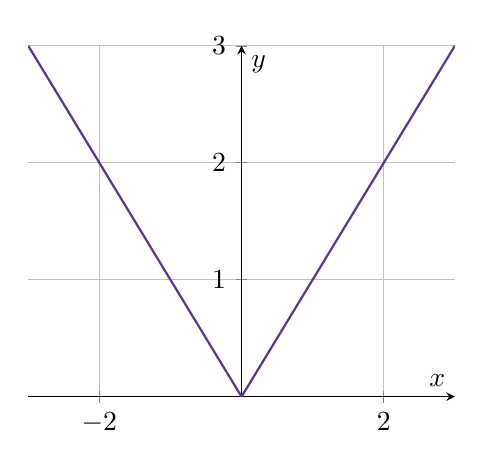
\begin{tikzpicture}
    \begin{axis}[
        grid=both,
        axis lines=middle,
        xmin=-3, xmax=3,
        ymin=0, ymax=3,
        xlabel={$x$},
        ylabel={$y$},
        ]
        \addplot[RoyalPurple, thick, domain=-3:3] {abs(x)};
    \end{axis}
\end{tikzpicture}
\end{minipage}
\hspace{1cm}
\begin{minipage}{0.4\textwidth}
\centering
\begin{tabular}{cc}

$x$ & $f(x)$ \\

-2 & 2 \\
-1 & 1 \\
0 & 0 \\
1 & 1 \\
2 & 2 \\

\end{tabular}
\end{minipage}
\noindent
The absolute value function $f(x) = |x|$ represents a \hl{V-shaped graph} that has its vertex at the origin (0,0). The function values are always non-negative, regardless of the sign of $x$.\\
\newpage
\section*{Unit 2: Rational Expressions}

\begin{lesson}{Lesson 1 - Review of Exponent Rules}
\textcolor{blue}{
The exponent rules are foundational principles that dictate how terms with the same base can be combined.
\begin{enumerate}
\item \(a^m \times a^n = a^{m+n}\) 
\item \(\frac{a^m}{a^n} = a^{m-n}\)
\item \((a^m)^n = a^{m \times n}\)
\end{enumerate}
}
\begin{example}
1. Using Rule 1: \(2^3 \times 2^4 = 2^{3+4} = 2^7\) \\
2. Using Rule 2: \(\frac{5^7}{5^4} = 5^{7-4} = 5^3\) \\
3. Using Rule 3: \((3^2)^3 = 3^{2 \times 3} = 3^6\)
\end{example}
\end{lesson}

\begin{lesson}{Lesson 2 - Rational Exponents}
\textcolor{blue}{
Rational exponents refer to exponents that are fractions. They can often be represented as roots.
\[
a^{\frac{m}{n}} = \sqrt[n]{a^m}
\]
}
\begin{example}
1. Using the formula: \(9^{\frac{1}{2}} = \sqrt[2]{9} = 3\) \\
2. \(16^{\frac{1}{4}} = \sqrt[4]{16} = 2\) \\
3. \(8^{\frac{2}{3}} = \sqrt[3]{8^2} = 4\)
\end{example}
\end{lesson}
\newpage
\begin{lesson}{Lesson 3 - Simplifying, Multiplying and Dividing Rational Expressions}
\textcolor{blue}{
Rational expressions are fractions wherein either the numerator, the denominator, or both are polynomials.
\begin{enumerate}
\item To multiply: Multiply the numerators with each other and the denominators with each other.
\item To divide: Multiply the first fraction by the reciprocal of the second.
\end{enumerate}
}
\begin{example}
1. Multiplication: \(\frac{x}{y} \times \frac{z}{w} = \frac{x \times z}{y \times w}\) \\
2. Division: \(\frac{x}{y} \div \frac{z}{w} = \frac{x}{y} \times \frac{w}{z}\) \\
3. Simplifying: \(\frac{3x}{6y} = \frac{x}{2y}\) \textcolor{red}{Divided by 2}
\end{example}
\end{lesson}

\begin{lesson}{Lesson 4 - Adding and Subtracting Rational Expressions}
\textcolor{blue}{
To add or subtract rational expressions:
\begin{enumerate}
\item Find a common denominator.
\item Rewrite each fraction with that denominator.
\item Add or subtract the numerators.
\end{enumerate}
}
\begin{example}
1. \(\frac{a}{c} + \frac{b}{d} = \frac{ad + bc}{cd}\) given that \(cd\) is the common denominator. \\
2. \(\frac{3x}{x^2-1} + \frac{2x}{x^2+2x} = \frac{3x(x+2) + 2x(x-1)}{x^2-1}\) \\
3. \(\frac{5}{x+3} - \frac{2}{x-2} = \frac{5(x-2) - 2(x+3)}{(x+3)(x-2)}\)
\end{example}
\end{lesson}

\begin{center}
\begin{tabular}{l l}
\textbf{Exponent Rule Name} & \textbf{Property} \\
\hline
Product Rule & \(a^x a^y = a^{x+y}\) \\
Negative Exponent & \(a^{-x} = \frac{1}{a^x}\) \\
Quotient Rule & \(\frac{a^x}{a^y} = a^{x-y}\) \\
Power of Power & \((a^x)^y = a^{xy}\) \\
Distributivity & \((ab)^x = a^x b^x\) \\
Fractional Exponent & \(a^{\frac{x}{y}} = \sqrt[y]{a^x}\) \\
\end{tabular}
\end{center}


\section*{\hl{Factoring Review}}
Factoring is the process of expressing a polynomial as a product of simpler polynomials. This document will demonstrate how to factor polynomials with examples and step-by-step explanations.

\begin{lesson}{Factoring Basics}
    To factor a polynomial, we look for common factors and apply various factoring techniques. Here are some common factoring methods:
\begin{enumerate}
    \item Factoring out the greatest common factor (GCF).
    \item Factoring by grouping.
    \item Factoring the difference of squares.
    \item Factoring trinomials of the form $ax^2 + bx + c$.
    \item Factoring special forms like the sum or difference of cubes.
\end{enumerate}

\end{lesson}


\begin{lesson}{Examples}
\end{lesson}
\begin{example}
Factoring the GCF.\\
Factor the polynomial $6x^2 + 12x$.
\begin{align*}
6x^2 + 12x &= 6x(x + 2) \quad \text{(Factor out the GCF, 6x)}
\end{align*}
\end{example}

\begin{example}
Factoring by Grouping.\\
Factor the polynomial $x^3 - x^2 + 4x - 4$.
\begin{align*}
x^3 - x^2 + 4x - 4 &= (x^3 - x^2) + (4x - 4) \quad \text{(Group the terms)} \\
&= x^2(x - 1) + 4(x - 1) \quad \text{(Factor out common factors)} \\
&= (x^2 + 4)(x - 1) \quad \text{(Factor further if possible)}
\end{align*}
\end{example}
\begin{example}
Factoring the Difference of Squares.\\
Factor the polynomial $9y^2 - 16z^2$.
\begin{align*}
9y^2 - 16z^2 &= (3y)^2 - (4z)^2 \quad \text{(Recognize it as a difference of squares)} \\
&= (3y + 4z)(3y - 4z) \quad \text{(Apply the difference of squares formula)}
\end{align*}
\end{example}
\begin{example}
Factoring a Trinomial.\\
Factor the trinomial $x^2 + 5x + 6$.

\begin{align*}
x^2 + 5x + 6 &= (x + 2)(x + 3) \quad \text{(Find two numbers that multiply to 6 and add up to 5)}
\end{align*}
\end{example}
\begin{example}
Factoring the Sum of Cubes.\\
Factor the polynomial $x^3 + 8$.
\begin{align*}
x^3 + 8 &= (x + 2)(x^2 - 2x + 4) \quad \text{(Recognize it as a sum of cubes)} \\
&= (x + 2)(x - 1 + 2i)(x - 1 - 2i) \quad \text{(Factor the quadratic using the quadratic formula)}
\end{align*}
\end{example}
\newpage 

\newpage
\section*{Unit 3: Quadratic Functions}
Quadratic functions are a class of polynomial functions of the form $f(x) = ax^2 + bx + c$, where $a$, $b$, and $c$ are constants, and $a$ is not equal to zero. They play a crucial role in algebra, calculus, physics, engineering, and various other fields. 
\section{The Standard Form of Quadratic Functions}

A quadratic function is typically expressed in standard form as:

\begin{equation}
f(x) = ax^2 + bx + c
\end{equation}

Here is a brief explanation of the parameters:

\begin{itemize}
    \item $a$: The coefficient of the quadratic term. It determines the direction in which the parabola opens (upwards if $a > 0$, and downwards if $a < 0$).
    \item $b$: The coefficient of the linear term. It shifts the vertex of the parabola horizontally.
    \item $c$: The constant term. It shifts the vertex of the parabola vertically.
\end{itemize}

\section{Vertex Form of a Quadratic Function}

The vertex form of a quadratic function is particularly useful for identifying the vertex and other properties. It is expressed as:

\begin{equation}
f(x) = a(x - h)^2 + k
\end{equation}

In this form, the vertex of the parabola is represented by the point $(h, k)$.
\newpage
\section{Vertex and Axis of Symmetry}

The vertex of a quadratic function in standard form ($f(x) = ax^2 + bx + c$) can be determined using the following formulas:

\begin{align}
x_{\text{vertex}} &= \frac{-b}{2a} \\
y_{\text{vertex}} &= f(x_{\text{vertex}})
\end{align}

In vertex form ($f(x) = a(x - h)^2 + k$), the vertex is already given as $(h, k)$.

The axis of symmetry is a vertical line that passes through the vertex. It is given by the equation:

\begin{equation}
x = \frac{-b}{2a}
\end{equation}

\section{Discriminant and Solutions}

Quadratic functions may have real or complex solutions. The discriminant ($\Delta$) can be used to determine the nature of the solutions:

\begin{equation}
\Delta = b^2 - 4ac
\end{equation}

The solutions are classified as follows:

\begin{itemize}
    \item If $\Delta > 0$, the function has two distinct real solutions.
    \item If $\Delta = 0$, the function has one real solution (a repeated root).
    \item If $\Delta < 0$, the function has two complex solutions.
\end{itemize}
\section{Graph of a Quadratic Function}

A graphical representation of a quadratic function helps us visualize its behavior. Let's consider an example:

\begin{equation}
f(x) = 2x^2 - 3x + 1
\end{equation}

\subsection{Vertex Calculation}

Using the formulas, we can find the vertex:

\begin{align*}
x_{\text{vertex}} &= \frac{-(-3)}{2(2)} = \frac{3}{4} \\
y_{\text{vertex}} &= f\left(\frac{3}{4}\right) = 2\left(\frac{3}{4}\right)^2 - 3\left(\frac{3}{4}\right) + 1 = \frac{7}{8}
\end{align*}

So, the vertex of the quadratic function is $\left(\frac{3}{4}, \frac{7}{8}\right)$.
\subsection{Graph}

You can visualize the graph of the quadratic function:

\begin{center}
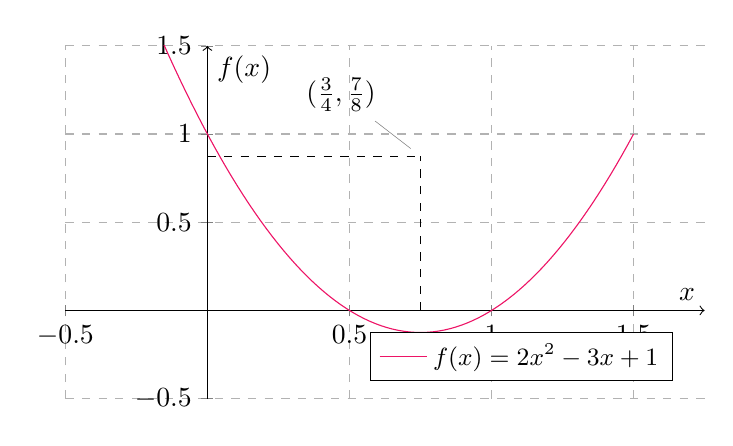
\begin{tikzpicture}
    \begin{axis}[
        xlabel=$x$,
        ylabel=$f(x)$,
        xmin=-0.5, xmax=1.75,
        ymin=-0.5, ymax=1.5,
        axis lines=middle,
        axis line style={->},
        legend style={at={(0.95,0.05)},anchor=south east},
        grid=both,
        major grid style={dashed,gray!60},
        width=0.8\textwidth,
        height=0.5\textwidth,
        legend style={font=\small},
        legend cell align={left},
    ]
    \addplot[WildStrawberry,domain=-0.5:1.5, samples=100] {2*x^2 - 3*x + 1};
    \legend{$f(x) = 2x^2 - 3x + 1$}
    
    \node[pin=135:{$(\frac{3}{4}, \frac{7}{8})$}] at (axis cs:0.75,0.875) {};
    \draw[dashed] (axis cs:0.75,0) -- (axis cs:0.75,0.875);
    \draw[dashed] (axis cs:0,0.875) -- (axis cs:0.75,0.875);
    
    \end{axis}
\end{tikzpicture}
\end{center}

\subsection*{\hl{Remember!}}

\begin{minipage}{\textwidth}
\textbf{Parabolas (Standard Form)}

\begin{tabularx}{\textwidth}{|X|X|}
\hline
\textbf{Equation} & $y = ax^2 + bx + c$ \\
\hline
\textbf{Vertex} & $(-\frac{b}{2a}, -\frac{b^2-4ac}{4a})$ \\
\hline
\textbf{Opening Direction} & Down if $a > 0$ \\
\hline
\textbf{Y-intercept} & $(0, c)$ \\
\hline
\end{tabularx}

\textbf{Parabolas (Vertex Form)}

\begin{tabularx}{\textwidth}{|X|X|}
\hline
\textbf{Equation} & $y = a(x - h)^2 + k$ \\
\hline
\textbf{Vertex} & $(h, k)$ \\
\hline
\textbf{Opening Direction} & Up if $a > 0$, Down if $a < 0$ \\
\hline
\end{tabularx}
\end{minipage}

\newpage
\section{Applications of Quadratic Functions}

Quadratic functions are not merely theoretical; they have numerous practical applications in various fields. Some common applications include:

\begin{enumerate}
    \item \textbf{Physics}: Quadratic functions describe the motion of objects under the influence of gravity. The equation $h(t) = -16t^2 + v_0t + h_0$ models the height ($h$) of an object at time ($t$) when it is thrown vertically with an initial velocity ($v_0$) from an initial height ($h_0$).

    \item \textbf{Engineering}: In structural engineering, quadratic equations model the deformation of materials under load, helping engineers design stable structures.

    \item \textbf{Economics}: Quadratic functions are used to model cost, revenue, and profit functions in business and economics. These functions assist in optimizing production and pricing strategies.

    \item \textbf{Computer Graphics}: In computer graphics, quadratic functions are used to create smooth curves and surfaces. For instance, Bézier curves are defined using quadratic equations.

    \item \textbf{Biology}: Quadratic functions can model population growth or decline of species. The logistic growth model is an example of such an application.

    \item \textbf{Statistics}: In regression analysis, quadratic functions are used to model complex relationships between variables.

    \item \textbf{Astronomy}: Quadratic equations can describe the orbits of celestial bodies and the motion of planets.

\end{enumerate}
\begin{note}
Quadratic functions are versatile and play a fundamental role in mathematics and various scientific disciplines. Understanding their properties, equations, and applications is crucial to problem solving and modeling real-world phenomena. Whether in physics, engineering, economics, or any other field, the knowledge of quadratic functions is a valuable asset in tackling complex problems.
\end{note}

\section*{Unit 4: Exponential Functions}
\begin{lesson}{1 - Exponential Growth}
\textcolor{blue}{Exponential growth} is a captivating concept where a quantity increases at a fixed percentage rate over time. This growth is modeled by the formula $y = ab^x$, where $a$ is the initial amount, $b$ is the growth factor, and $x$ is the time variable.

\begin{example}
Suppose you invest $1000$ at an annual interest rate of $5\%$, compounded annually. The growth formula is $A = 1000 \times (1 + 0.05)^x$. After 3 years, the amount would be approximately $A = 1000 \times (1 + 0.05)^3 \approx 1157.63$.
\end{example}

\begin{note}
The graph of an exponential growth function is characterized by a distinct upward curve that becomes steeper as $b$ increases.

\begin{center}
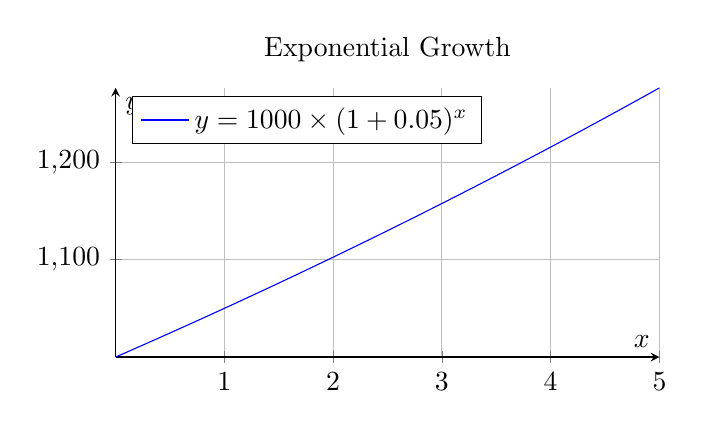
\begin{tikzpicture}
\begin{axis}[
  xlabel=$x$,
  ylabel=$y$,
  grid=major,
  axis lines=middle,
  width=0.7\linewidth,
  height=5cm,
  title={Exponential Growth},
  legend pos=north west,
]
\addplot[blue, domain=0:5, samples=100, smooth] {1000 * (1 + 0.05)^x};
\addlegendentry{$y = 1000 \times (1 + 0.05)^x$}
\end{axis}
\end{tikzpicture}
\end{center}
\end{note}
\end{lesson}
\newpage
\begin{lesson}{2 - Exponential Decay}
\textcolor{blue}{Exponential decay} is the counterpart to exponential growth. It occurs when a quantity decreases at a fixed percentage rate over time. The decay is modeled by the formula $y = ab^x$, where $b$ is between 0 and 1.

\begin{example}
Consider a radioactive substance that decays at a rate of 10\% per year. Its decay formula is $N = N_0 \times 0.9^t$. After 5 years, the remaining quantity is $N = N_0 \times 0.9^5$.
\end{example}

\begin{note}
The graph of an exponential decay function exhibits a decreasing curve that approaches but never reaches zero.

\begin{center}
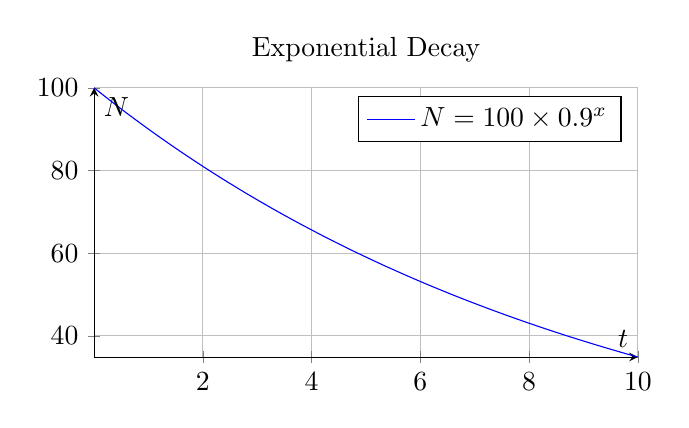
\begin{tikzpicture}
\begin{axis}[
  xlabel=$t$,
  ylabel=$N$,
  grid=major,
  axis lines=middle,
  width=0.7\linewidth,
  height=5cm,
  title={Exponential Decay},
  legend pos=north east,
]
\addplot[blue, domain=0:10, samples=100, smooth] {100 * 0.9^x};
\addlegendentry{$N = 100 \times 0.9^x$}
\end{axis}
\end{tikzpicture}
\end{center}
\end{note}
\end{lesson}
\newpage
\begin{lesson}{3 - Compound Interest}
\textcolor{blue}{Compound interest} is a powerful concept where interest is added to the initial principal, which then earns interest over time. The compound interest formula is given by $A = P(1 + r/n)^{nt}$, where $A$ is the final amount, $P$ is the principal, $r$ is the annual interest rate, $n$ is the number of times interest is compounded per year, and $t$ is the time in years.

\begin{example}
Imagine investing $5000$ at an annual interest rate of $6\%$, compounded quarterly. The formula is $A = 5000 \times (1 + 0.06/4)^{4t}$. After 2 years, the amount is $A = 5000 \times (1 + 0.06/4)^{4 \times 2}$.
\end{example}

\begin{note}
Compound interest enables your investment to grow faster compared to simple interest, especially with more frequent compounding.
\end{note}
\end{lesson}
\newpage 
\begin{lesson}{4 - Properties of Exponential Functions}
\textcolor{blue}{Exponential functions} possess several key properties:

\begin{itemize}
    \item They have a constant base.
    \item They can model growth or decay.
    \item They have an asymptote, which they approach but never reach.
    \item They are always positive if the base is greater than 1.
    \item They are always decreasing if the base is between 0 and 1.
\end{itemize}

\begin{example}
Consider the function $f(x) = 2^x$. It has a constant base of 2 and models exponential growth.
\end{example}

\begin{note}
The graph of an exponential function approaches but never crosses the horizontal axis (asymptote).

\begin{center}
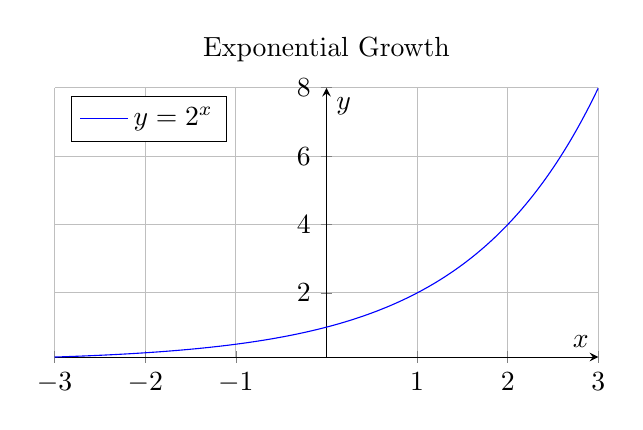
\begin{tikzpicture}
\begin{axis}[
  xlabel=$x$,
  ylabel=$y$,
  grid=major,
  axis lines=middle,
  width=0.7\linewidth,
  height=5cm,
  title={Exponential Growth},
  legend pos=north west,
]
\addplot[blue, domain=-3:3, samples=100, smooth] {2^x};
\addlegendentry{$y = 2^x$}
\end{axis}
\end{tikzpicture}
\end{center}
\end{note}
\end{lesson}
\newpage 
\begin{lesson}{5 - Transformations}
\textcolor{blue}{Transformations} offer a way to modify the graph of an exponential function. Common transformations include vertical shifts, horizontal shifts, reflections, and stretches or compressions. These transformations are applied to the base function $y = b^x$.

\begin{example}
If $g(x) = 3 \times 2^x$, the function $g$ is a vertical stretch of $f(x) = 2^x$ by a factor of 3.
\end{example}

\begin{note}
Transformations alter the appearance and behavior of the exponential function graph.

\begin{center}
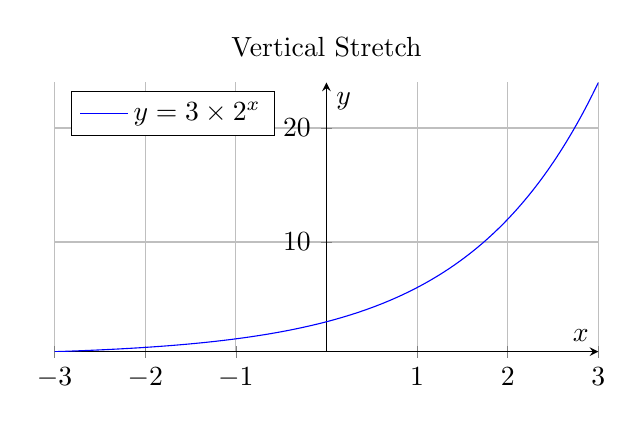
\begin{tikzpicture}
\begin{axis}[
  xlabel=$x$,
  ylabel=$y$,
  grid=major,
  axis lines=middle,
  width=0.7\linewidth,
  height=5cm,
  title={Vertical Stretch},
  legend pos=north west,
]
\addplot[blue, domain=-3:3, samples=100, smooth] {3 * 2^x};
\addlegendentry{$y = 3 \times 2^x$}
\end{axis}
\end{tikzpicture}
\end{center}
Transformations can also involve horizontal shifts, reflections, and other modifications to customize the behavior of the exponential function graph.
\end{note}
\end{lesson}



\newpage
\begin{lesson}{6 - Applications of Exponential Functions}
\textcolor{blue}{Exponential functions} find applications in various real-world scenarios, such as population growth, radioactive decay, and financial investments. Understanding these applications is crucial for solving problems in science, economics, and other fields.

\begin{example}
Population growth can be modeled using the exponential function $P(t) = P_0 \times (1 + r)^t$, where $P(t)$ is the population at time $t$, $P_0$ is the initial population, $r$ is the growth rate, and $t$ is time.
\end{example}

\begin{example}
Radioactive decay is a common application where the decay of a substance is modeled by the function $N(t) = N_0 \times e^{-kt}$, where $N(t)$ is the remaining quantity at time $t$, $N_0$ is the initial quantity, $k$ is the decay constant, and $t$ is time.
\end{example}

\begin{example}
Financial investments often involve compound interest, and the amount of money accumulated over time is given by the formula $A = P(1 + r/n)^{nt}$, where $A$ is the final amount, $P$ is the principal, $r$ is the annual interest rate, $n$ is the number of times interest is compounded per year, and $t$ is time in years.
\end{example}
\end{lesson}
\newpage
\begin{lesson}{7 - Summative Assessment }
\begin{enumerate}
    \item \textbf{Evaluate the following:}
    \begin{enumerate}[label=\alph*)]
        \item $2^3$:
        \begin{align*}
            2^3 &= 2 \times 2 \times 2 \\
            &= 8
        \end{align*}
        
        \item $10^{-2}$:
        \begin{align*}
            10^{-2} &= \frac{1}{10^2} \\
            &= \frac{1}{100} \\
            &= 0.01
        \end{align*}
        
        \item $e^0$:
        \begin{align*}
            e^0 &= 1
        \end{align*}
    \end{enumerate}
    
    \item \textbf{Solve for $x$:}
    \begin{enumerate}[label=\alph*)]
        \item $5^x = 125$:
        \begin{align*}
            5^x &= 125 \\
            x &= 3
        \end{align*}
        
        \item $2e^{2x} = 16$:
        \begin{align*}
            e^{2x} &= 8 \\
            2x &= \ln(8) \\
            x &= \frac{\ln(8)}{2}
        \end{align*}
    \end{enumerate}
\newpage
    \item \textbf{Consider the function $f(x) = 3 \times 2^x$. Perform the following transformations and sketch the resulting graph:}
    \begin{enumerate}[label=\alph*)]
        \item \textbf{Vertical stretch by a factor of 2:}
        The function becomes $g(x) = 6 \times 2^x$.
        
        \item \textbf{Horizontal shift right by 1 unit:}
        The function becomes $h(x) = 3 \times 2^{(x - 1)}$.
        
        \item \textbf{Reflection across the $x$-axis:}
        The function becomes $k(x) = -3 \times 2^x$.
        
        \textbf{Graph:} (Note: This is a conceptual sketch; precise plotting requires numerical values.)

\definecolor{lessonbgcolor}{rgb}{0.9,0.9,1}
\definecolor{examplecolor}{rgb}{0.8,1,0.8}
\definecolor{blue}{RGB}{0,70,170}

\pgfplotsset{
    compat=1.17,
    every axis/.append style={
        axis line style={->},
        xlabel style={anchor=west},
        ylabel style={anchor=south},
        legend style={at={(0.03,0.97)}, anchor=north west, draw=none, fill=none, font=\scriptsize},
    },
}


\begin{figure}[h]
    \centering
    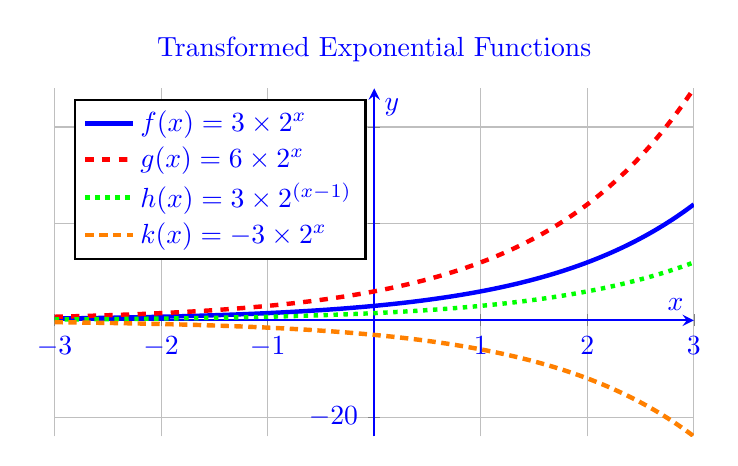
\begin{tikzpicture}
        \begin{axis}[
            xlabel={$x$},
            ylabel={$y$},
            grid=major,
            axis lines=middle,
            width=0.8\linewidth,
            height=6cm,
            title={Transformed Exponential Functions},
            legend pos=north west,
            domain=-3:3,
            samples=100,
            smooth,
            % Adjust the style of each plot
            blue,
            thick,
            every axis plot/.append style={ultra thick},
            legend cell align=left,
        ]
            \addplot [blue] {3 * 2^x};
            \addlegendentry{$f(x) = 3 \times 2^x$}
            
            \addplot [red, dashed] {6 * 2^x};
            \addlegendentry{$g(x) = 6 \times 2^x$}
            
            \addplot [green, dotted] {3 * 2^(x - 1)};
            \addlegendentry{$h(x) = 3 \times 2^{(x - 1)}$}
            
            \addplot [orange, densely dashed] {-3 * 2^x};
            \addlegendentry{$k(x) = -3 \times 2^x$}
        \end{axis}
    \end{tikzpicture}
    \caption{Transformed Exponential Functions}
    \label{fig:transformed-exponential}
\end{figure}
    \end{enumerate}
\end{enumerate}
\end{lesson}

\newpage
\subsection*{Resources}
\begin{itemize}
    \item \href{https://www.jensenmath.ca/math11-review}{Grade 11 Review - Jensen Math}
    \item \href{https://sites.google.com/a/hdsb.ca/mrturingia/home/grade-11-university-math}{Grade 11 University Math- Textbook solution}
    \item \href{https://app.prepanywhere.com/student/prep/textbooks/11-functions-harcourt}{PrepAnywhere}
\end{itemize}
\end{document}
